%definira klasu dokumenta 
\documentclass[12pt]{report} 

%prostor izmedu naredbi \documentclass i \begin{document} se zove uvod. U njemu se nalaze naredbe koje se odnose na cijeli dokument

%osnovni LaTex ne može riješiti sve probleme, pa se koriste različiti paketi koji olakšavaju izradu željenog dokumenta
\usepackage[croatian]{babel} 
\usepackage{amssymb}
\usepackage{amsmath}
\usepackage{txfonts}
\usepackage{mathdots}
\usepackage{titlesec}
\usepackage{array}
\usepackage{lastpage}
\usepackage{etoolbox}
\usepackage{longtable, tabu}
\usepackage{color, colortbl}
\usepackage{adjustbox}
\usepackage{geometry}
\usepackage[classicReIm]{kpfonts}
\usepackage{hyperref}
\usepackage{fancyhdr}

\usepackage{float}
\usepackage{setspace}
\restylefloat{table}


\patchcmd{\chapter}{\thispagestyle{plain}}{\thispagestyle{fancy}}{}{} %redefiniranje stila stranice u paketu fancyhdr

%oblik naslova poglavlja
\titleformat{\chapter}{\normalfont\huge\bfseries}{\thechapter.}{20pt}{\Huge}
\titlespacing{\chapter}{0pt}{0pt}{40pt}


\linespread{1.3} %razmak između redaka

\geometry{a4paper, left=1in, top=1in,}  %oblik stranice

\hypersetup{ colorlinks, citecolor=black, filecolor=black, linkcolor=black,	urlcolor=black }   %izgled poveznice


%prored smanjen između redaka u nabrajanjima i popisima
\newenvironment{packed_enum}{
	\begin{enumerate}
		\setlength{\itemsep}{0pt}
		\setlength{\parskip}{0pt}
		\setlength{\parsep}{0pt}
	}{\end{enumerate}}

\newenvironment{packed_item}{
	\begin{itemize}
		\setlength{\itemsep}{0pt}
		\setlength{\parskip}{0pt}
		\setlength{\parsep}{0pt}
	}{\end{itemize}}


%boja za privatni i udaljeni kljuc u tablicama
\definecolor{LightBlue}{rgb}{0.9,0.9,1}
\definecolor{LightGreen}{rgb}{0.9,1,0.9}


%podesavanje zaglavlja i podnožja

\pagestyle{fancy}
\lhead{Programsko inženjerstvo}
\rhead{$<$Projektni zadatak$>$}
\lfoot{$<$Naziv grupe$>$}
\cfoot{stranica \thepage/\pageref{LastPage}}
\rfoot{\today}
\renewcommand{\headrulewidth}{0.2pt}
\renewcommand{\footrulewidth}{0.2pt}


\begin{document} 
	
	
	
	\begin{titlepage}
		\begin{center}
			\vspace*{\stretch{1.0}} %u kombinaciji s ostalim \vspace naredbama definira razmak između redaka teksta
			\LARGE Programsko inženjerstvo\\
			\large Ak. god. 2020./2021.\\
			
			\vspace*{\stretch{3.0}}
			
			\huge $<$Naziv projekta$>$\\
			\Large Dokumentacija, Rev. \textit{$<$1 ili 2$>$}\\
			
			\vspace*{\stretch{12.0}}
			\normalsize
			Grupa: \textit{$<$Naziv grupe$>$}\\
			Voditelj: \textit{$<$Ime i prezime voditelja$>$}\\
			
			
			\vspace*{\stretch{1.0}}
			Datum predaje: \textit{$<$dan$>$. $<$mjesec$>$. $<$godina$>$.}\\
	
			\vspace*{\stretch{4.0}}
			
			Nastavnik: \textit{$<$Ime i prezime nastavnika zaduženog za vašu grupu$>$}\\
		
		\end{center}

	
	\end{titlepage}

	
	\tableofcontents

	\chapter{Dnevnik promjena dokumentacije}
		
		\textbf{\textit{Kontinuirano osvježavanje}}\\
				
		
		\begin{longtabu} to \textwidth {|X[2, l]|X[13, l]|X[3, l]|X[3, l]|}
			\hline \multicolumn{1}{|l|}{\textbf{Rev.}}	& \multicolumn{1}{l|}{\textbf{Opis promjene/dodatka}} & \multicolumn{1}{|l|}{\textbf{Autori}} & \multicolumn{1}{l|}{\textbf{Datum}} \\[3pt] \hline
			\endfirsthead
			
			\hline \multicolumn{1}{|l|}{\textbf{Rev.}}	& \multicolumn{1}{l|}{\textbf{Opis promjene/dodatka}} & \multicolumn{1}{|l|}{\textbf{Autori}} & \multicolumn{1}{l|}{\textbf{Datum}} \\[3pt] \hline
			\endhead
			
			\hline 
			\endlastfoot
			
			0.1 & Dodani dionici i aktori i opisano prvih 8 \textit{Use Case} dijagrama & Jukanović & 09.11.2020. \\[3pt] \hline 
			0.2 & Dodan dijagram obrasca uporabe (funkcionalnost prijavljenog korisnika) & Jukanović & 10.11.2020 \\[3pt] \hline 
			0.3 & Dodano još 7 (09-15) \textit{Use Case} dijagrama & Brstilo & 10.11.2020. \\[3pt] \hline
			0.4 & Modificirani zahtjevi aktora i dodani (16-25) \textit{Use case} dijagrama & Antunović & 10.11.2020. \\[3pt] \hline 
			0.5 & Dodan dijagram obrasca uporabe (funkcionalnost administratora) & Antunović & 11.11.2020. \\[3pt] \hline 
			0.6 & Dodan dijagram razreda generičke funkcionalnosti &  Cigula & 12.11.2020.\\[3pt] \hline 
			0.7 & Dodani sekvencijski dijagrami & Marošević & 13.11.2020. \\[3pt] \hline 
			0.8 & Dodana arhitektura baze podataka & Piškur, Marošević & 13.11.2020.  \\[3pt] \hline 
			0.9 & Dodani arhitektura sustava, opis projektnog zadatka i ostali zahtjevi & Rončević & 13.11.2020. \\[3pt] \hline 
			\textbf{1.0} & Korigiranje teksta i provjera dokumentacije & Marošević, Cigula, Jukanović & 13.11.2020 \\[3pt] \hline  
			1.1 & Dodan dijagram razmještaja & Jukanović & 11.01.2021 \\[3pt] \hline
			1.2 & Dodani dijagrami aktivnosti & Antunović & 13.01.2021. \\[3pt] \hline 
			1.3 & Dodan dijagram stanja & Jukanović & 13.01.2021. \\[3pt] \hline 
			1.4 & Modificirani modeli baze podataka & Antunović & 14.01.2021 \\[3pt] \hline 
			1.5 & Dodan dijagram razreda  & Cigula  & 14.01.2021  \\[3pt] \hline 
		  	1.6 & Dodane slike koda pod ispitivanje komponenti & Cigula  & 14.01.2021  \\[3pt] \hline 
			1.7 & Ažurirani sati rada i dnevnik sastajanja & Cigula & 14.01.2021  \\[3pt] \hline 
			 1.8 & Dodana uputstva za puštanje u pogon & Marošević  & 14.01.2021. \\[3pt] \hline 
			 1.9 & Dodani zaključak, korištene tehnologije i ispitivanje sustava & Rončević & 14.01.2021. \\[3pt] \hline 
			 1.10 & Dodan dijagram komponenti &Piškur  & 14.01.2021. \\[3pt] \hline 
			 &  &  &  \\[3pt] \hline
			
			
		\end{longtabu}
	
	
		\textit{Moraju postojati glavne revizije dokumenata 1.0 i 2.0 na kraju prvog i drugog ciklusa. Između tih revizija mogu postojati manje revizije već prema tome kako se dokument bude nadopunjavao. Očekuje se da nakon svake značajnije promjene (dodatka, izmjene, uklanjanja dijelova teksta i popratnih grafičkih sadržaja) dokumenta se to zabilježi kao revizija. Npr., revizije unutar prvog ciklusa će imati oznake 0.1, 0.2, …, 0.9, 0.10, 0.11.. sve do konačne revizije prvog ciklusa 1.0. U drugom ciklusu se nastavlja s revizijama 1.1, 1.2, itd.}

	\chapter{Opis projektnog zadatka}
		
		
		\indent Cilj ovog projekta je razviti programsku podršku za stvaranje web aplikacije "Maketa shop" koja se sastoji od dva glavna dijela. 
		\indent Prvi dio omogućuje objavljivanje sadržaja vezanih uz izradu maketa. Sadržaj je u obliku priča koje se sastoje od slika, videa, teksta ili kombinacija svega navedenog koji prate proces izrade maketa. Same priče objavljuje administrator dok registrirani korisnici iste mogu predlagati. Postoji mogućnost dodavanja komentara na priče, koje mogu ostavljati registrirani i neregistrirani korisnici. \\
		\indent Drugi dio je \textit{webshop} na kojemu korisnici mogu naručivati makete. Sam \textit{shop} je standardna web-trgovina sa svim funkcionalnostima koje korisnik očekuje od takve stranica. Razlika između "Maketa shopa" i drugih web-trgovina je u mogućnosti naručivanja maketa po vlastitim zamislima. Korisnik može maketaru (administratoru) poslati nacrte i opise makete kakvu želi, a maketar taj zahtjev može prihvatiti ili odbiti. Kada se obje strane slože oko cijene, proces se nastavlja na standardan način.
		
		\begin{figure}[H]
			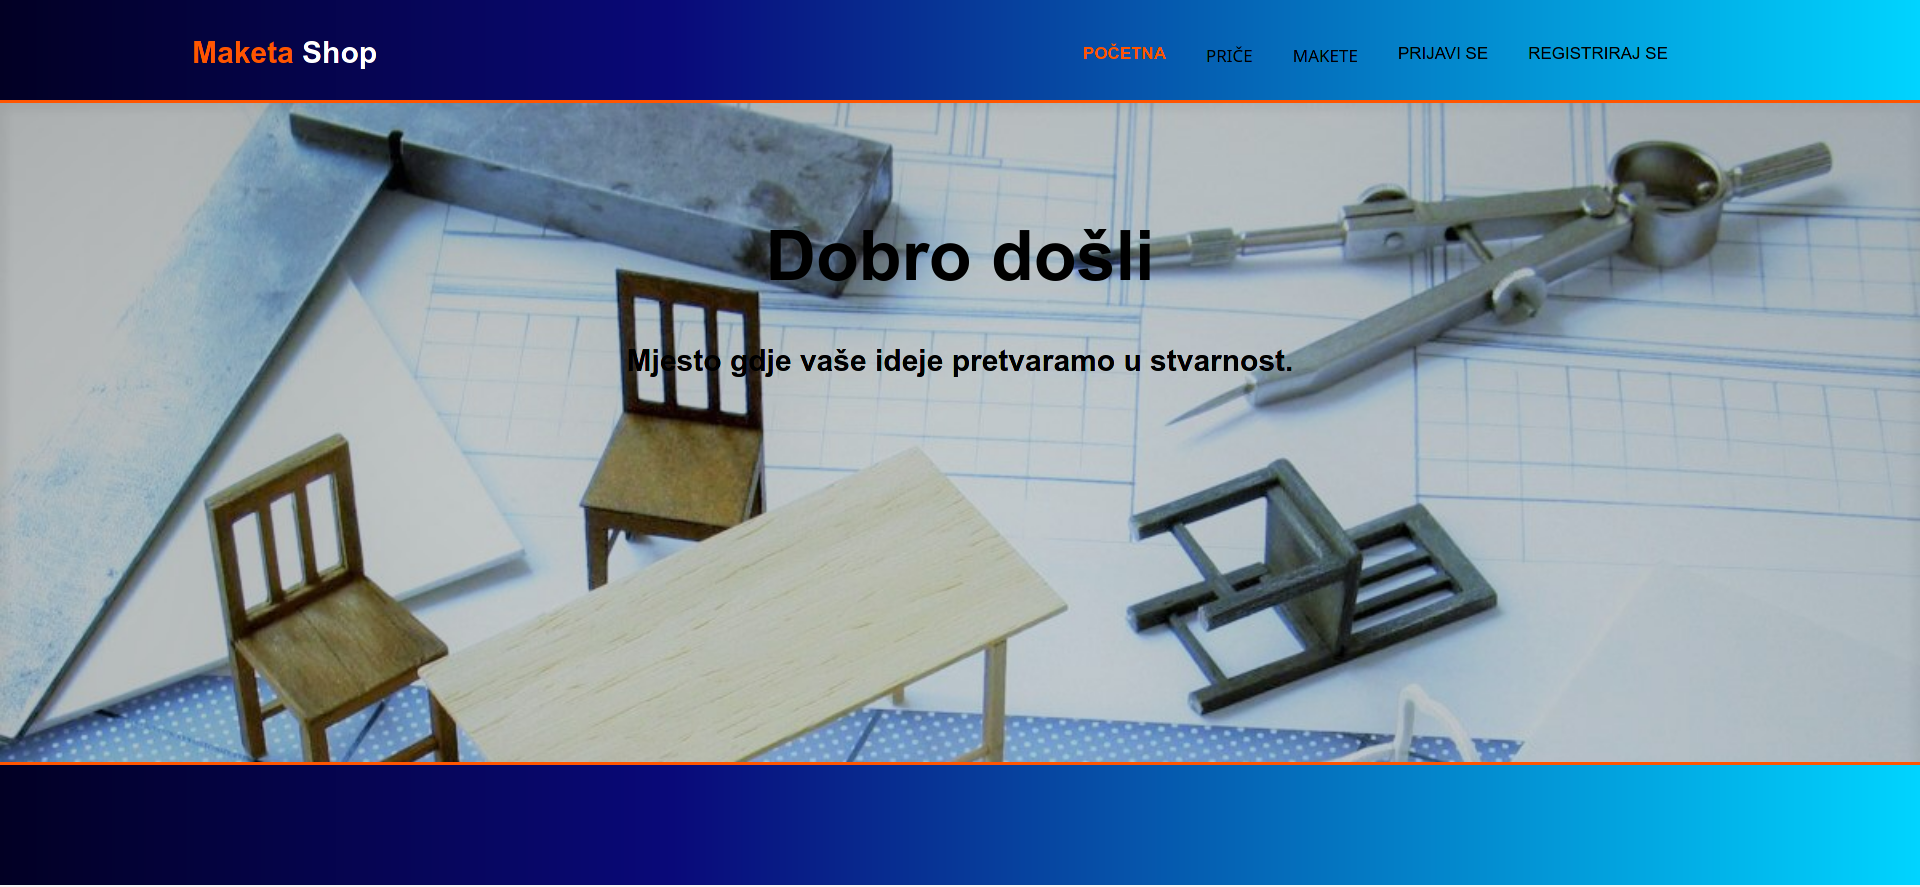
\includegraphics[width=.9\linewidth]{slike/20201112_182209.png}
			\centering
			\caption{Početna stranica}
			\label{fig:opis1}
		\end{figure}
	
		Aplikaciji mogu pristupiti registrirani i neregistrirani korisnici. Pri prvom ulasku u aplikaciju, svaki korisnik ima opciju Registracije, te prijavljivanja s postojećim računom. Aplikacija registriranim korisnicima pruža mogućnost spremanja informacija kako se ne bi trebali svaki put prijavljivati i unositi osobne podatke prilikom plaćanja narudžbe. Podaci potrebni za kreiranje korisničkog računa su:
		
		\begin{itemize}
			\item korisničko ime (mora biti jedinstveno)
			\item e-mail adresa (mora biti jedinstvena)
			\item lozinka
		\end{itemize} 	
	
		\begin{figure}[H]
			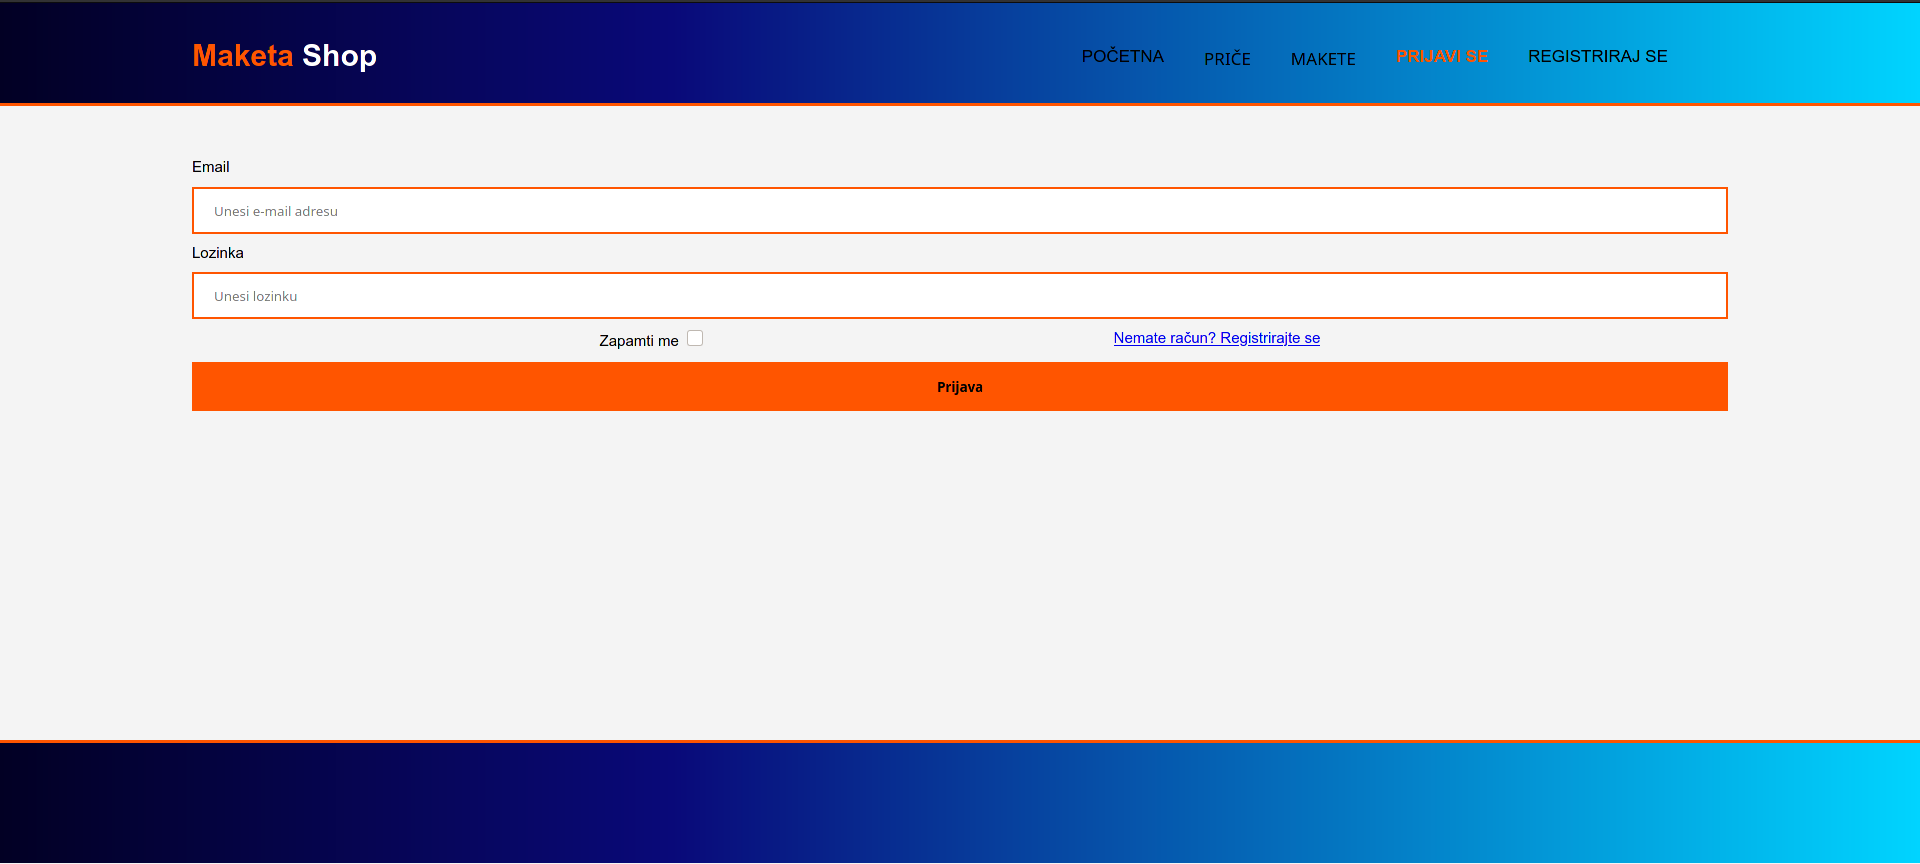
\includegraphics[width=.9\linewidth]{slike/20201112_182228.png}
			\centering
			\caption{Prijava u sustav}
			\label{fig:opis2}
		\end{figure}
	
		\begin{figure}[H]
			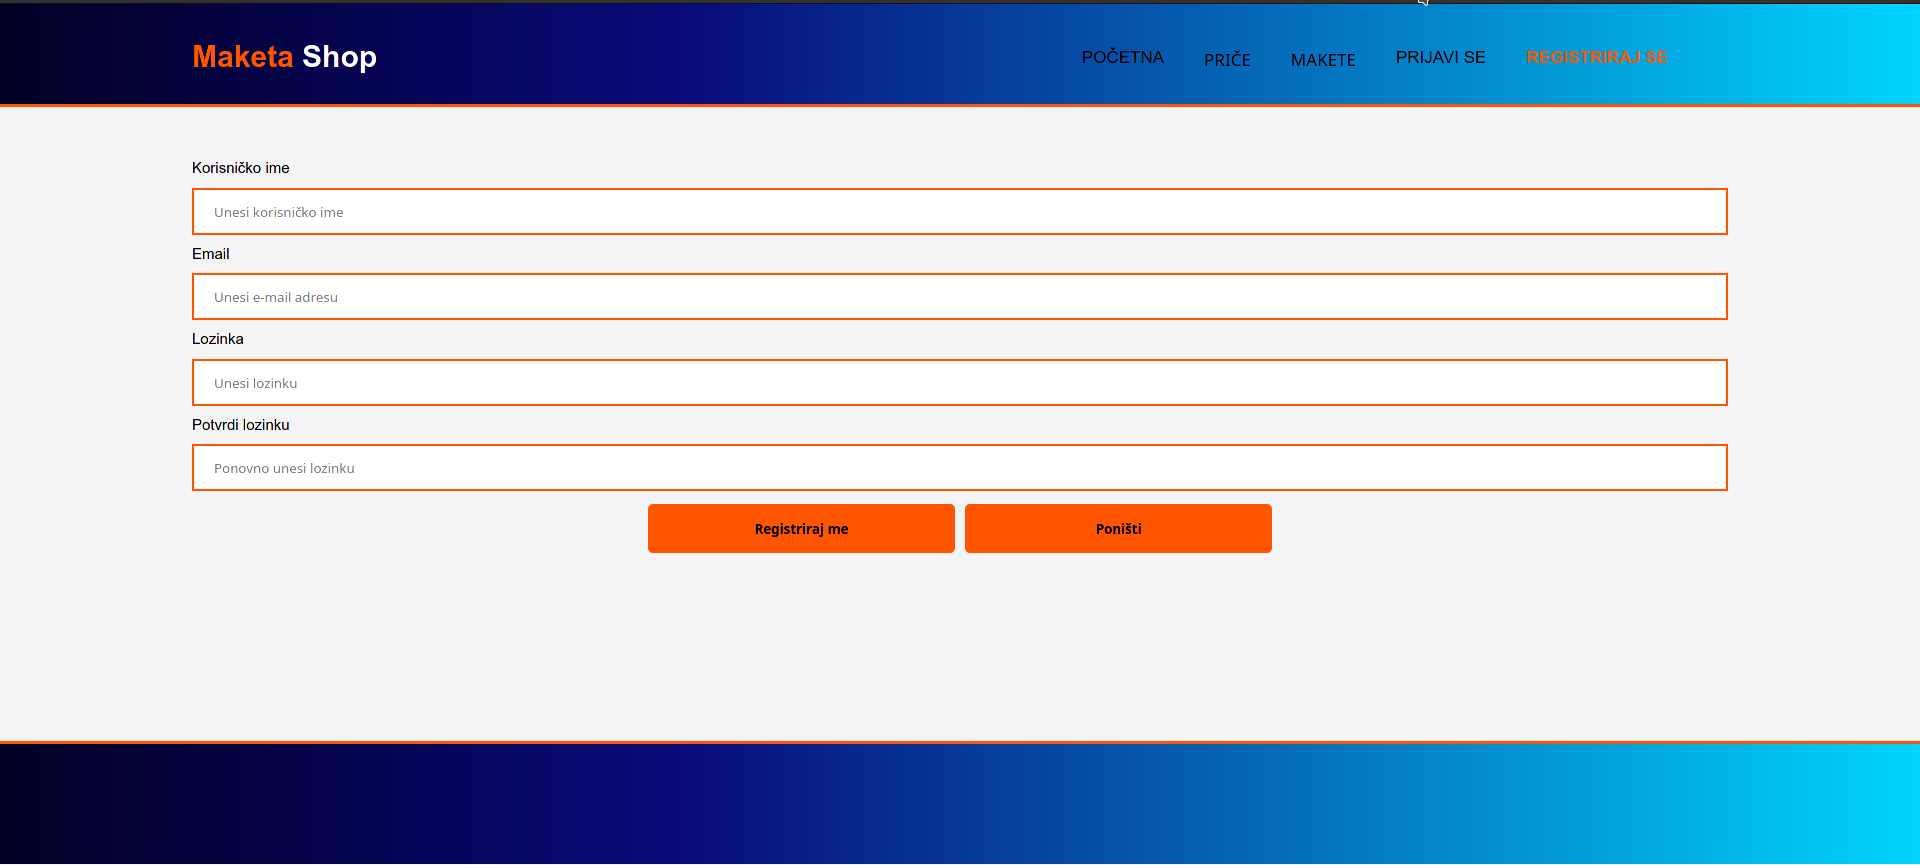
\includegraphics[width=.9\linewidth]{slike/20201112_182312.png}
			\centering
			\caption{Registracija}
			\label{fig:opis3}
		\end{figure}
	
		Korisničko ime je javno svima dok za druge podatke korisnik određuje hoće li biti privatni ili javni.\\
		
		Aplikacija pruža opciju kupnju standardne makete. Svaka maketa je detaljno opisana (dimenzija, materijal, boja) te se korisniku pruža mogućnost odabira nekoliko različitih materijala koji bi se koristili u izradi makete. Cijene će se razlikovati ovisno o biranim materijalima, te su one unaprijed određene od strane administratora. Također korisniku je omogućeno naručivanje makete prema vlastitim skicama. Atributi makete će se unositi u formular gdje se definira opis makete, dimenzija i materijal za izradu. Nakon što se formular ispuni administratoru se šalje obavijest, te ona ima mogućnost pregleda zahtjeva te određuje cijenu za tu maketu, koju korisnik može prihvatiti ili odbiti. \\
		Plaćanje se 'odvija' pomoću formulara čijim se ispunjavanjem simulira online plaćanje. Podaci uneseni u formular se trebaju spremati, te se registriranim korisnicima nakon prvog plaćanja formular automatski puni. Povijest svih transakcija se treba spremati i pamtiti te mora biti dostupna administratoru. \\
		
		Postoje 3 vrste korisnika u aplikaciji:
		\begin{itemize}
			\item \underline{Neregistrirani korisnik} je osnovna uloga u web aplikaciji. Neregistrirani korisnik ima mogućnost kupovine maketa, međutim njegovi podaci se neće automatski popunjavati prilikom svake sljedeće kupovine, omogućeno mu je komentiranje na postojeće priče međutim nema mogućnosti predlaganja novih priča.
			\item \underline{Registrirani korisnik} je uloga koja se ostvaruje prilikom registracije i prijave. Registrirani korisnik ima sve mogućnosti kao i neregistrirani korisnik međutim za njega postoji mogućnost automatskog ispunjavanja podataka prilikom plaćanja, te mogućnost predlaganja priča administratoru, također ima mogućnost naručivanja maketa prema vlastitim specifikacijama.
			\item \underline{Administrator} je uloga koja se dodjeljuje jednoj osobi te on ima najveće ovlasti. Administrator je jedina osoba koja može objavljivati priče, samostalno ili na prijedlog registriranih korisnika. Također ima mogućnost pregleda proteklih transakcija. Administratoru je omogućena zabrana pristupa registriranim korisnicima.
		\end{itemize}
	\chapter{Specifikacija programske potpore}
		
	\section{Funkcionalni zahtjevi}
			
			\noindent \textbf{Dionici:}
			
			\begin{packed_enum}
				
				\item Korisnik sustava
				\begin{packed_enum}	
					\item  Maketar 
					\item  Kupac	
				\end{packed_enum}
				\item Administrator	sustava			
				\item Razvojni tim
				
			\end{packed_enum}
			
			\noindent \textbf{Aktori i njihovi funkcionalni zahtjevi:}
			
			
			\begin{packed_enum}
				\item  \underbar{Neregistrirani/neprijavljeni korisnik (inicijator) može:}
				
				\begin{packed_enum}
					
					\item registrirati se u sustav prilaganjem svoje e-mail adrese, lozinke i korisničkog imena
					\item pregledati priče i ostavljati komentare na njima
					\item unijeti podatke za kupovinu i kupiti proizvod
					\item pregledati makete i izabrati materijal makete
						
				\end{packed_enum}
					
				
				\item  \underbar{Korisnik (kupac/maketar) može:}
				
				\begin{packed_enum}
					
					\item pregledati priče i ostavljati komentare na njima
					\item pregledati makete i izabrati materijal makete
					\item slati administratoru sustava prijedloge za nove priče
					\item slati administratoru sustava zahtjev za maketu po narudžbi
					\item prihvaćati ili odbijati ponudu cijene za maketu po narudžbi
					\item vidjeti podatke o svom korisničkom računu
					\item postavljati vidljivost svojih podataka
					\item kupiti proizvod
					\item odjaviti se
					
				\end{packed_enum}
				

			
			\item  \underbar{Administrator (inicijator) može:}
			
			\begin{packed_enum}
				
				\item prihvaćati ili odbijati prijedloge priča
				\item prihvaćanjem objavljivati predložene priče
				\item ponuditi cijenu za maketu po narudžbi
				\item vidjeti podatke o izvršenim transakcijama
				\item zabraniti pristup registriranim korisnicima
				\item postavljati makete standardne ponude
				
			\end{packed_enum}
			

		
		\item  \underbar{Baza podataka (sudionik) može:}
		
		\begin{packed_enum}
			
			\item pohranjivati podatke o svim korisničkim računima sustava i njihovim ovlastima
			\item pohranjivati priče i njihove dane opise
			\item pohranjivati makete
			\item pohranjivati podatke za plaćanje
			\item pohranjivati zahtjeve za maketama
			\item pohranjivati ponude cijena za makete 
			\item pohranjivati stanje vidljivosti podataka korisnika
			\item pohranjivati podatke o izvršenim transakcijama
			\item pohranjivati podatke o korisnicima sa zabranjenim pristupom
			\item pohranjivati podatke maketa standardne ponude 
			
		\end{packed_enum}
		\end{packed_enum}
			
			\eject 
			
			
				
			\subsection{Obrasci uporabe}
				
				\subsubsection{Opis obrazaca uporabe}
							
						\noindent \underbar{\textbf{UC1 $-$ Registracija}}
					\begin{packed_item}
						
						\item \textbf{Glavni sudionik: }Korisnik
						\item  \textbf{Cilj:} Napraviti korisnički račun za korisnika
						\item  \textbf{Sudionici:} Baza podataka
						\item  \textbf{Preduvjet:} -
						\item  \textbf{Opis osnovnog tijeka:}
						
						\item[] \begin{packed_enum}
							
							\item Neregistrirani korisnik odabire opciju za registraciju
							\item Unosi potrebne podatke za registraciju
							\item Korisnikovi podaci se upisuju u bazu te je obaviješten o uspješnoj registraciji
						\end{packed_enum}
						
						\item  \textbf{Opis mogućih odstupanja:}
						
						\item[] \begin{packed_item}
							
							\item[2.a] Odabir već zauzetog korsiničkog imena i/ili e-maila, unos podataka u nedozvoljenom formatu (npr. lozinka) ili pružanje neispravnog e-maila
							\item[] \begin{packed_enum}
								
								\item Korisnik je obaviješten o nastaloj grešci i mjestu na kojem se ona nalazi
								\item Korisnik potom ispravlja grešku i ponovo šalje podatke ili odustaje od registracije
								
							\end{packed_enum}					
						\end{packed_item}
					\end{packed_item}
				
						\noindent \underbar{\textbf{UC2 $-$ Pregled priča}}
					\begin{packed_item}
						
						\item \textbf{Glavni sudionik: }Korisnik
						\item  \textbf{Cilj:} Korisniku se pruža stranica sa kratkim prikazom svih priča u sustavu
						\item  \textbf{Sudionici:} Baza podataka
						\item  \textbf{Preduvjet:} -
						\item  \textbf{Opis osnovnog tijeka:}
						
						\item[] \begin{packed_enum}
							
							\item Korisnik sa početne stranice poveznicom dolazi do stranice sa pričama
							\item Aplikacija korisniku prikazuje sve priče u sustavu
						\end{packed_enum}
					\end{packed_item}
				
						\noindent \underbar{\textbf{UC3 $-$ Pregled pojedine priče}}
					\begin{packed_item}
						
						\item \textbf{Glavni sudionik: }Korisnik
						\item  \textbf{Cilj:} Korisniku se pruža detaljan prikaz određene priče
						\item  \textbf{Sudionici:} Baza podataka
						\item  \textbf{Preduvjet:} -
						\item  \textbf{Opis osnovnog tijeka:}
						
						\item[] \begin{packed_enum}
							
							\item Korisnik iz kratkog prikaza priča odabire priču koja ga zanima
							\item Aplikacija korisniku pruža detaljan prikaz priče (slika, video, tekst) i mogućnost komentiranja na priču
						\end{packed_enum}
					\end{packed_item}
				
						\noindent \underbar{\textbf{UC4 $-$ Komentiranje priče}}
					\begin{packed_item}
						
						\item \textbf{Glavni sudionik: }Korisnik
						\item  \textbf{Cilj:} Korisnik sustava ostavlja komentar na priču 
						\item  \textbf{Sudionici:} Baza podataka
						\item  \textbf{Preduvjet:} -
						\item  \textbf{Opis osnovnog tijeka:}
						
						\item[] \begin{packed_enum}
							\item Korisnik otvara priču na kojoj želi ostaviti komentar
							\item U za to namijenjeno mjesto upisuje komentar te ga objavljuje
							\item Komentar se objavljuje te je uz njega navedeno ime korisnika koji ga je objavio
							\item 
						\end{packed_enum}
						
						\item  \textbf{Opis mogućih odstupanja:}
						
						\item[] \begin{packed_item}
							
							\item[3.a] Korisnik nije prijavljen u sustav
							\item[] \begin{packed_enum}
								
								\item Umjesto korisničkog imena na to mjesto se upisuje $"$Anoniman korisnik$"$
								
							\end{packed_enum}
							\item[2.b] $<$opis mogućeg scenarija odstupanja u koraku 2$>$
							\item[3.a] $<$opis mogućeg scenarija odstupanja  u koraku 3$>$
							
						\end{packed_item}
					\end{packed_item}
				
						\noindent \underbar{\textbf{UC5 $-$ Predlaganje priče}}
					\begin{packed_item}
						
						\item \textbf{Glavni sudionik: }Korisnik
						\item  \textbf{Cilj:} Korisnik šalje prijedlog priče za objavu na stranici administratoru 
						\item  \textbf{Sudionici:} Administrator, baza podataka
						\item  \textbf{Preduvjet:} Korisnik je prijavljen u sustav
						\item  \textbf{Opis osnovnog tijeka:}
						
						\item[] \begin{packed_enum}
							
							\item Korisnik iz izbornika odabire opciju predlaganja priče
							\item Aplikacija mu pruža sučelje za dodavanje opisa priče (slika, video, tekst)
							\item Korisnik popunjava podatke i šalje ih administratoru na pregled
						\end{packed_enum}
						
						\item  \textbf{Opis mogućih odstupanja:}
						
						\item[] \begin{packed_item}
							
							\item[2.a] Korisnik nije predao dovoljno podataka (nema ni slike, ni teksta, ni videa i/ili nema naslova) 
							\item[] \begin{packed_enum}
								
								\item Korisnik je obaviješten o grešci i mjestu na kojem je nastala
								\item Korisnik ispravlja grešku i šalje podatke administratoru na pregled ili odustaje od slanja prijedloga priče								
							\end{packed_enum}			
						\end{packed_item}
					\end{packed_item}
				
					\noindent \underbar{\textbf{UC6 $-$ Prilaganje slike/teksta/videa priči}}
				\begin{packed_item}
					
					\item \textbf{Glavni sudionik: }Korisnik
					\item  \textbf{Cilj:} Opisivanje priče koja se predlaže administratoru tekstom, slikom i videom
					\item  \textbf{Sudionici:} Baza podataka
					\item  \textbf{Preduvjet:} Korisnik je prijavljen u sustav
					\item  \textbf{Opis osnovnog tijeka:}
					
					\item[] \begin{packed_enum}
						
						\item Korisniku je pružen upravljač kojim dodaje proizvoljan broj elemenata teksta, slike i videa 
						\item Korisnik u elemente upisuje tekst ili prilaže sliku ili video ili ih uklanja
						\item Nakon što je popunio podatke, može ih slati administratoru
					\end{packed_enum}
					
					\item  \textbf{Opis mogućih odstupanja:}
					
					\item[] \begin{packed_item}
						
						\item[2.a] Korisnik prilaže sliku ili video nedozvoljenog formata
						\item[] \begin{packed_enum}
							
							\item Korisnik je obaviješten o grešci i dano mu je pojašnjenje te greške
							\item Korisnik odustaje od prilaganja slike/videa uz priču ili prilaže sliku/video u drugom formatu
							
						\end{packed_enum}	
					\end{packed_item}
				\end{packed_item}
			
					\noindent \underbar{\textbf{UC7 $-$ Odobrenje/odbijanje priče}}
				\begin{packed_item}
					
					\item \textbf{Glavni sudionik: }Administrator
					\item  \textbf{Cilj:} Predložena priča se objavljuje na za to predviđenoj stranici ili se odbacuje
					\item  \textbf{Sudionici:} Baza podataka
					\item  \textbf{Preduvjet:} Korisnik je prijavljen i dodana su mu prava administratora
					\item  \textbf{Opis osnovnog tijeka:}
					
					\item[] \begin{packed_enum}
						
						\item Aplikacija administratoru pruža listu priča danih na prijedlog i njihov opis
						\item Administratoru je ispod svake priče ponuđena opcija odbacivanja ili prihvaćanja priče
						\item Priča se ovisno o administratorovom izboru uklanja iz sustava ili se objavljuje
					\end{packed_enum}
				\end{packed_item}
			
					\noindent \underbar{\textbf{UC8 $-$ Objava priče}}
				\begin{packed_item}
					
					\item \textbf{Glavni sudionik: }Administrator
					\item  \textbf{Cilj:} Priča se nakon korisnikog odobravanja prikazuje svim korisnicima sustava na za to određenom mjestu
					\item  \textbf{Sudionici:} Baza podataka
					\item  \textbf{Preduvjet:} Korisnik je prijavljen u sustav i dodana su mu prava administratora
					\item  \textbf{Opis osnovnog tijeka:}
					
					\item[] \begin{packed_enum}
						
						\item Administrator prihvaća priču
						\item Priča se pohranjuje u bazu podataka te se prikazuje na određenoj stranici zajedno sa ostalim pričama
					\end{packed_enum}
				\end{packed_item}
				
					\noindent \underbar{\textbf{UC9 $-$ Prijava}}
				\begin{packed_item}
					
					\item \textbf{Glavni sudionik: }Korisnik
					\item  \textbf{Cilj:} Prijaviti korisnika u sustav
					\item  \textbf{Sudionici:} Baza podataka
					\item  \textbf{Preduvjet:} Korisnik je registriran u bazi podataka
					\item  \textbf{Opis osnovnog tijeka:}
						
					\item[] \begin{packed_enum}
							
						\item Neprijavljen korisnik odabire opciju za prijavu
						\item Unosi potrebne podatke za prijavu
						\item Podaci se provjeravaju u bazi podataka te se obavještava o uspješnoj prijavi
					\end{packed_enum}
						
					\item  \textbf{Opis mogućih odstupanja:}
						
					\item[] \begin{packed_item}
							
						\item[2.a] Unos nepostojećeg korisničkog imena ili e-maila, unos pogrešne lozinke
						\item[] \begin{packed_enum}
								
							\item Korisnik je obaviješten o nastaloj grešci i mjestu na kojem se ona nalazi
							\item Korisnik potom ispravlja grešku i ponovo šalje podatke ili odustaje od prijave
								
						\end{packed_enum}					
					\end{packed_item}
				\end{packed_item}
				
					\noindent \underbar{\textbf{UC10 $-$ Odjava}}
				\begin{packed_item}
					
					\item \textbf{Glavni sudionik: }Korisnik
					\item  \textbf{Cilj:} Odjaviti se iz sustava
					\item  \textbf{Sudionici:} -
					\item  \textbf{Preduvjet:} Korisnik je prijavljen u sustav
					\item  \textbf{Opis osnovnog tijeka:}
					
					\item[] \begin{packed_enum}
						
						\item Prijavljen korisnik odabire opciju za odjavu 
						\item Obavještava se korisnika o uspješnoj odjavi
					\end{packed_enum}
				\end{packed_item}
				
					\noindent \underbar{\textbf{UC11 $-$ Prikaz korisničkog računa}}
				\begin{packed_item}
					
					\item \textbf{Glavni sudionik: }Korisnik
					\item  \textbf{Cilj:} Prikazati podatke o korisničkom računu
					\item  \textbf{Sudionici:} Baza podataka
					\item  \textbf{Preduvjet:} Korisnik je prijavljen u sustav
					\item  \textbf{Opis osnovnog tijeka:}
					
					\item[] \begin{packed_enum}
						
						\item Prijavljen korisnik odabire opciju za prikaz svog korisničkog računa 
						\item Prikazuju se podaci o korisničkom računu
					\end{packed_enum}
				\end{packed_item}
				
					\noindent \underbar{\textbf{UC12 $-$ Unos podataka za kupovinu za prijavljenog korisnika}}
				\begin{packed_item}
					
					\item \textbf{Glavni sudionik: }Korisnik
					\item  \textbf{Cilj:} Popuniti formular za kupovinu makete
					\item  \textbf{Sudionici:} Baza podataka
					\item  \textbf{Preduvjet:} Korisnik je prijavljen u bazi podataka
					\item  \textbf{Opis osnovnog tijeka:}
						
					\item[] \begin{packed_enum}
							
						\item Prijavljen korisnik odabire opciju za kupnju makete
						\item Formular s podacima za kupovinu se automatski ispuni osobnim podacima
						\item Odabire se opcija za izvršavanje transakcije/kupnje
						\item Obavještava se korisnika o uspješnoj transakciji/kupnji
					\end{packed_enum}
				\end{packed_item}
				
					\noindent \underbar{\textbf{UC13 $-$ Unos podataka za kupovinu za neregistriranog korisnika}}
				\begin{packed_item}
					
					\item \textbf{Glavni sudionik: }Korisnik
					\item  \textbf{Cilj:} Popuniti formular za kupovinu makete
					\item  \textbf{Sudionici:} Baza podataka
					\item  \textbf{Preduvjet:} -
					\item  \textbf{Opis osnovnog tijeka:}
						
					\item[] \begin{packed_enum}
							
						\item Neregistrirani korisnik odabire opciju za kupnju makete
						\item Ispunjava formular za kupovinu s osobnim podacima
						\item Odabire se opcija za izvršavanje transakcije/kupnje
						\item Obavještava se korisnika o uspješnoj transakciji/kupnji
					\end{packed_enum}
						
					\item  \textbf{Opis mogućih odstupanja:}
						
					\item[] \begin{packed_item}
							
						\item[2.a] Unos pogrešnih osobnih podataka ili podataka potrebnih za transakciju
						\item[] \begin{packed_enum}
								
							\item Korisnik je obaviješten o nastaloj grešci i mjestu na kojem se ona nalazi
							\item Korisnik potom ispravlja grešku i ponovo šalje podatke ili odustaje od kupnje
								
						\end{packed_enum}					
					\end{packed_item}
				\end{packed_item}
				
					\noindent \underbar{\textbf{UC14 $-$ Spremanje izvršenih transakcija}}
				\begin{packed_item}
					
					\item \textbf{Glavni sudionik: }Baza podataka
					\item  \textbf{Cilj:} Spremiti izvršene transakcije u bazu podataka
					\item  \textbf{Sudionici:} -
					\item  \textbf{Preduvjet:} Transakcija je uspješno obavljena
					\item  \textbf{Opis osnovnog tijeka:}
						
					\item[] \begin{packed_enum}
							
						\item Sustav javlja korisniku da je transakcija uspješna
						\item Baza podataka sprema podatke o transakciji
					\end{packed_enum}
				\end{packed_item}
				
					\noindent \underbar{\textbf{UC15 $-$ Pregled izvršenih transakcija}}
				\begin{packed_item}
					
					\item \textbf{Glavni sudionik: }Administrator
					\item  \textbf{Cilj:} Pregled podataka o izvršenim transakcijama
					\item  \textbf{Sudionici:} Baza podataka
					\item  \textbf{Preduvjet:} Korisnik je prijavljen u sustav i dodana su mu prava administratora
					\item  \textbf{Opis osnovnog tijeka:}
						
					\item[] \begin{packed_enum}
							
						\item Administrator odabire opciju za pregled prošlih transakcija
						\item Prikazuju se podaci iz baze podataka o transakcijama
					\end{packed_enum}
				\end{packed_item}
			
					\noindent \underbar{\textbf{UC16 $-$ Pregled maketa}}
				\begin{packed_item}
				
					\item \textbf{Glavni sudionik: }Korisnik
					\item  \textbf{Cilj:} Korisniku se pruža stranica s kratkim prikazom svih maketa u sustavu
					\item  \textbf{Sudionici:} Baza podataka
					\item  \textbf{Preduvjet:} -
					\item  \textbf{Opis osnovnog tijeka:}
					
					\item[] \begin{packed_enum}
					
						\item Korisnik s početne stranice poveznicom dolazi do stranice s maketama
						\item Aplikacija korisniku prikazuje sve makete u sustavu
					\end{packed_enum}
				\end{packed_item}
			
			
					\noindent \underbar{\textbf{UC17 $-$ Pregled pojedine makete}}
				\begin{packed_item}
					
					\item \textbf{Glavni sudionik: }Korisnik
					\item  \textbf{Cilj:} Korisniku se pruža detaljan prikaz pojedine makete
					\item  \textbf{Sudionici:} Baza podataka
					\item  \textbf{Preduvjet:} -
					\item  \textbf{Opis osnovnog tijeka:}
					
					\item[] \begin{packed_enum}
						
						\item Korisnik sa stranice s pregledom svih maketa odabire maketu koja ga zanima
						\item Aplikacija korisniku prikazuje detaljan opis tražene makete koji uključuje tekst, slike, izbornike te mogućnost kupovine makete
					\end{packed_enum}
				\end{packed_item}
			
				\noindent \underbar{\textbf{UC18 $-$ Odabir materijala za maketu}}
				\begin{packed_item}
					
					\item \textbf{Glavni sudionik: }Korisnik
					\item  \textbf{Cilj:} Korisniku se pruža mogućnost odabira materijala od kojeg želi da se izradi maketa
					\item  \textbf{Sudionici:} Baza podataka
					\item  \textbf{Preduvjet:} Korisnik mora biti na stranici pojedinačne makete
					\item  \textbf{Opis osnovnog tijeka:}
					
					\item[] \begin{packed_enum}
						
						\item Korisnik na stranici makete otvara padajući izbornik s opcijama za materijale te odabire željeni materijal
						\item Aplikacija na osnovu odabranog materijala izračunava cijenu makete te prikazuje novu cijenu na stranici
					\end{packed_enum}
				\end{packed_item}
				
				
				\noindent \underbar{\textbf{UC19 $-$ Spremanje podataka formulara za plaćanje}}
				\begin{packed_item}
					
					\item \textbf{Glavni sudionik: }Korisnik
					\item  \textbf{Cilj:} Formular koji je ispunio registrirani korisnik pri plaćanju se sprema za ponovno korištenje
					\item  \textbf{Sudionici:} Baza podataka
					\item  \textbf{Preduvjet:} Korisnik mora biti registriran te ispravno popuniti formular
					\item  \textbf{Opis osnovnog tijeka:}
					
					\item[] \begin{packed_enum}
						
						\item Korisnik na stranici za plaćanje ispunjava formular
						\item Aplikacija provjerava ispravnost unesenih podataka
						\item Nakon provjere podatci se spremaju u bazu podataka za ponovnu upotrebu pri sljedećoj kupovini
					\end{packed_enum}
				
					\item  \textbf{Opis mogućih odstupanja:}
					
					\item[] \begin{packed_item}
						
						\item[2.a] Korisnik neispravno popuni jedno ili više polja ili ostavi prazno polje
						\item[] \begin{packed_enum}
							
							\item Korisnik je obaviješten o grešci i dano mu je pojašnjenje te greške
							\item Korisnik prepravlja ili nadopunjava podatke te se oni ponovno šalju na validaciju ili odustaje od ispunjavanja formulara
							
						\end{packed_enum}	
					\end{packed_item}
				\end{packed_item}
			
				\noindent \underbar{\textbf{UC20 $-$ Popunjavanje formulara za maketu po narudžbi}}
				\begin{packed_item}
					
					\item \textbf{Glavni sudionik: }Korisnik
					\item  \textbf{Cilj:} Korisnik predaje formular sa specifikacijama željene makete 
					\item  \textbf{Sudionici:} Baza podataka, administrator
					\item  \textbf{Preduvjet:} Korisnik mora biti registriran te ispravno popuniti formular
					\item  \textbf{Opis osnovnog tijeka:}
					
					\item[] \begin{packed_enum}
						
						\item Korisnik na stranici za ispunjavanje formulara popunjava formular sa željenim dimenzijama, materijalom i opisom
						\item Aplikacija provjerava ispravnost unesenih podataka
						\item Nakon provjere podatci se spremaju u bazu podataka
						\item Administratoru se šalje obavijest o novom formularu
					\end{packed_enum}
					
					\item  \textbf{Opis mogućih odstupanja:}
					
					\item[] \begin{packed_item}
 
						\item[2.a] Korisnik neispravno popuni jedno ili više polja ili ostavi prazno polje
						\item[] \begin{packed_enum}
							
							\item Korisnik je obaviješten o grešci i dano mu je pojašnjenje te greške
							\item Korisnik prepravlja ili nadopunjava podatke te se oni ponovno šalju na validaciju ili odustaje od ispunjavanja formulara
							
						\end{packed_enum}	
					\end{packed_item}
				\end{packed_item}


				\noindent \underbar{\textbf{UC21 $-$ Ponuda makete na zahtjev}}
				\begin{packed_item}
					
					\item \textbf{Glavni sudionik: }Administrator
					\item  \textbf{Cilj:} Administrator pregledava zahtjev te šalje ponudu na osnovu traženih specifikacija
					\item  \textbf{Sudionici:} Baza podataka, korisnik
					\item  \textbf{Preduvjet:} Administrator mora imati predan zahtjev od strane korisnika
					\item  \textbf{Opis osnovnog tijeka:}
					
					\item[] \begin{packed_enum}
						
						\item Administrator dobija obavijest o podnesenom zahtjevu te otvara zahtjev
						\item Administrator na osnovu zahtjeva određuje cijenu te šalje ponudu korisniku
						\item Korisnik dobija obavijest o ponudi
					\end{packed_enum}
				\end{packed_item}

				\noindent \underbar{\textbf{UC22 $-$ Prihvat ili odbijanje ponude makete}}
				\begin{packed_item}
					
					\item \textbf{Glavni sudionik: }Korisnik
					\item  \textbf{Cilj:} Korisnik prihvaća ili odbija ponuđenu cijenu makete
					\item  \textbf{Sudionici:} Baza podataka, administrator
					\item  \textbf{Preduvjet:} Korisnik mora biti registriran
					\item  \textbf{Opis osnovnog tijeka:}
					
					\item[] \begin{packed_enum}
						
						\item Korisnik dobija obavijest o ponudi cijene za maketu
						\item Korisnik odbija ili prihvaća ponudu
						\item Šalje se povratna informacija administratoru
					\end{packed_enum}
				\end{packed_item}

				\noindent \underbar{\textbf{UC23 $-$ Postavljanje postavki vidljivosti korisničkog računa}}
				\begin{packed_item}
					
					\item \textbf{Glavni sudionik: }Korisnik
					\item  \textbf{Cilj:} Korisnik postavlja željenu vidljivost svojih podataka
					\item  \textbf{Sudionici:} Baza podataka
					\item  \textbf{Preduvjet:} Korisnik mora biti registriran
					\item  \textbf{Opis osnovnog tijeka:}
					
					\item[] \begin{packed_enum}
						
						\item Korisnik odabire stranicu s postavkama korisničkog računa
						\item Korisnik odabire opciju postavljanja vidljivosti
						\item Korisnik odabire stavke koje želi da budu privatne ili javne (korisničko ime mora biti javno)
						\item Korisnik potvrđuje odabir te se on šalje sustavu
						\item Stranica osvježava podatke
					\end{packed_enum}

					\item  \textbf{Opis mogućih odstupanja:}
					
					\item[] \begin{packed_item}
 
						\item[4.a] Korisnik ne potvrdi svoj odabir prije napuštanja stranice
						\item[] \begin{packed_enum}
							
							\item Korisnik je obaviješten o grešci te se nudi opcija povratka na potvrdu odabira
							\item Korisnik potvrđuje ili odustaje od izmjena
							
						\end{packed_enum}	
					\end{packed_item}
				\end{packed_item}

				\noindent \underbar{\textbf{UC24 $-$ Zabrana pristupa korisniku}}
				\begin{packed_item}
					
					\item \textbf{Glavni sudionik: }Administrator
					\item  \textbf{Cilj:} Administrator zabranjuje pristup određenom registriranom korisniku
					\item  \textbf{Sudionici:} Baza podataka, korisnik
					\item  \textbf{Preduvjet:} Korisnik mora biti registriran
					\item  \textbf{Opis osnovnog tijeka:}
					
					\item[] \begin{packed_enum}
						
						\item Administrator odabire korisnika kojem želi zabraniti pristup
						\item Potvrđuje odabir te se sprema u bazu podataka
					\end{packed_enum}
				\end{packed_item}


				\noindent \underbar{\textbf{UC25 $-$ Kreiranje standardne ponude maketa}}
				\begin{packed_item}
					
					\item \textbf{Glavni sudionik: }Administrator
					\item  \textbf{Cilj:} Administrator ispunjava i objavljuje standardnu ponudu na stranici
					\item  \textbf{Sudionici:} Baza podataka
					\item  \textbf{Preduvjet:} -
					\item  \textbf{Opis osnovnog tijeka:}
					
					\item[] \begin{packed_enum}
						
						\item Administrator ispunjava podatke za novu ponudu makete
						\item Administrator potvrđuje formular te se šalje u bazu podataka
						\item Nova maketa se sprema te se počinje prikazivati na stranici
					\end{packed_enum}

					\item  \textbf{Opis mogućih odstupanja:}
					
					\item[] \begin{packed_item}
 
						\item[2.a] Administrator krivo ispuni ili ostavi prazno polje u formularu
						\item[] \begin{packed_enum}
							
							\item Administrator je obaviješten o grešci te se nudi opcija povratka na ispunjavanje formulara
							\item Korisnik izmjenjuje ili nadopunjava podatke te ponovno potvrđuje odabir
							
						\end{packed_enum}	
					\end{packed_item}
				\end{packed_item}
			
			\noindent \underbar{\textbf{UC26 $-$ Kupnja makete}}
			\begin{packed_item}
				
				\item \textbf{Glavni sudionik: }Korisnik
				\item  \textbf{Cilj:} Korisniku se nudi obrazac koji služi za popunjavanje podataka potrebnih za kupnju
				\item  \textbf{Sudionici:} Baza podataka
				\item  \textbf{Preduvjet:} -
				\item  \textbf{Opis osnovnog tijeka:}
				
				\item[] \begin{packed_enum}
					
					\item Korisnik sa stranice makete odabire opciju kupnje nje
					\item Korisniku se prikazuje obrazac u kojem popunjava ili provjerava podatke za kupnju
				\end{packed_enum}
			\end{packed_item}
					
				\subsubsection{Dijagrami obrazaca uporabe}
					
					\begin{figure}[H]
						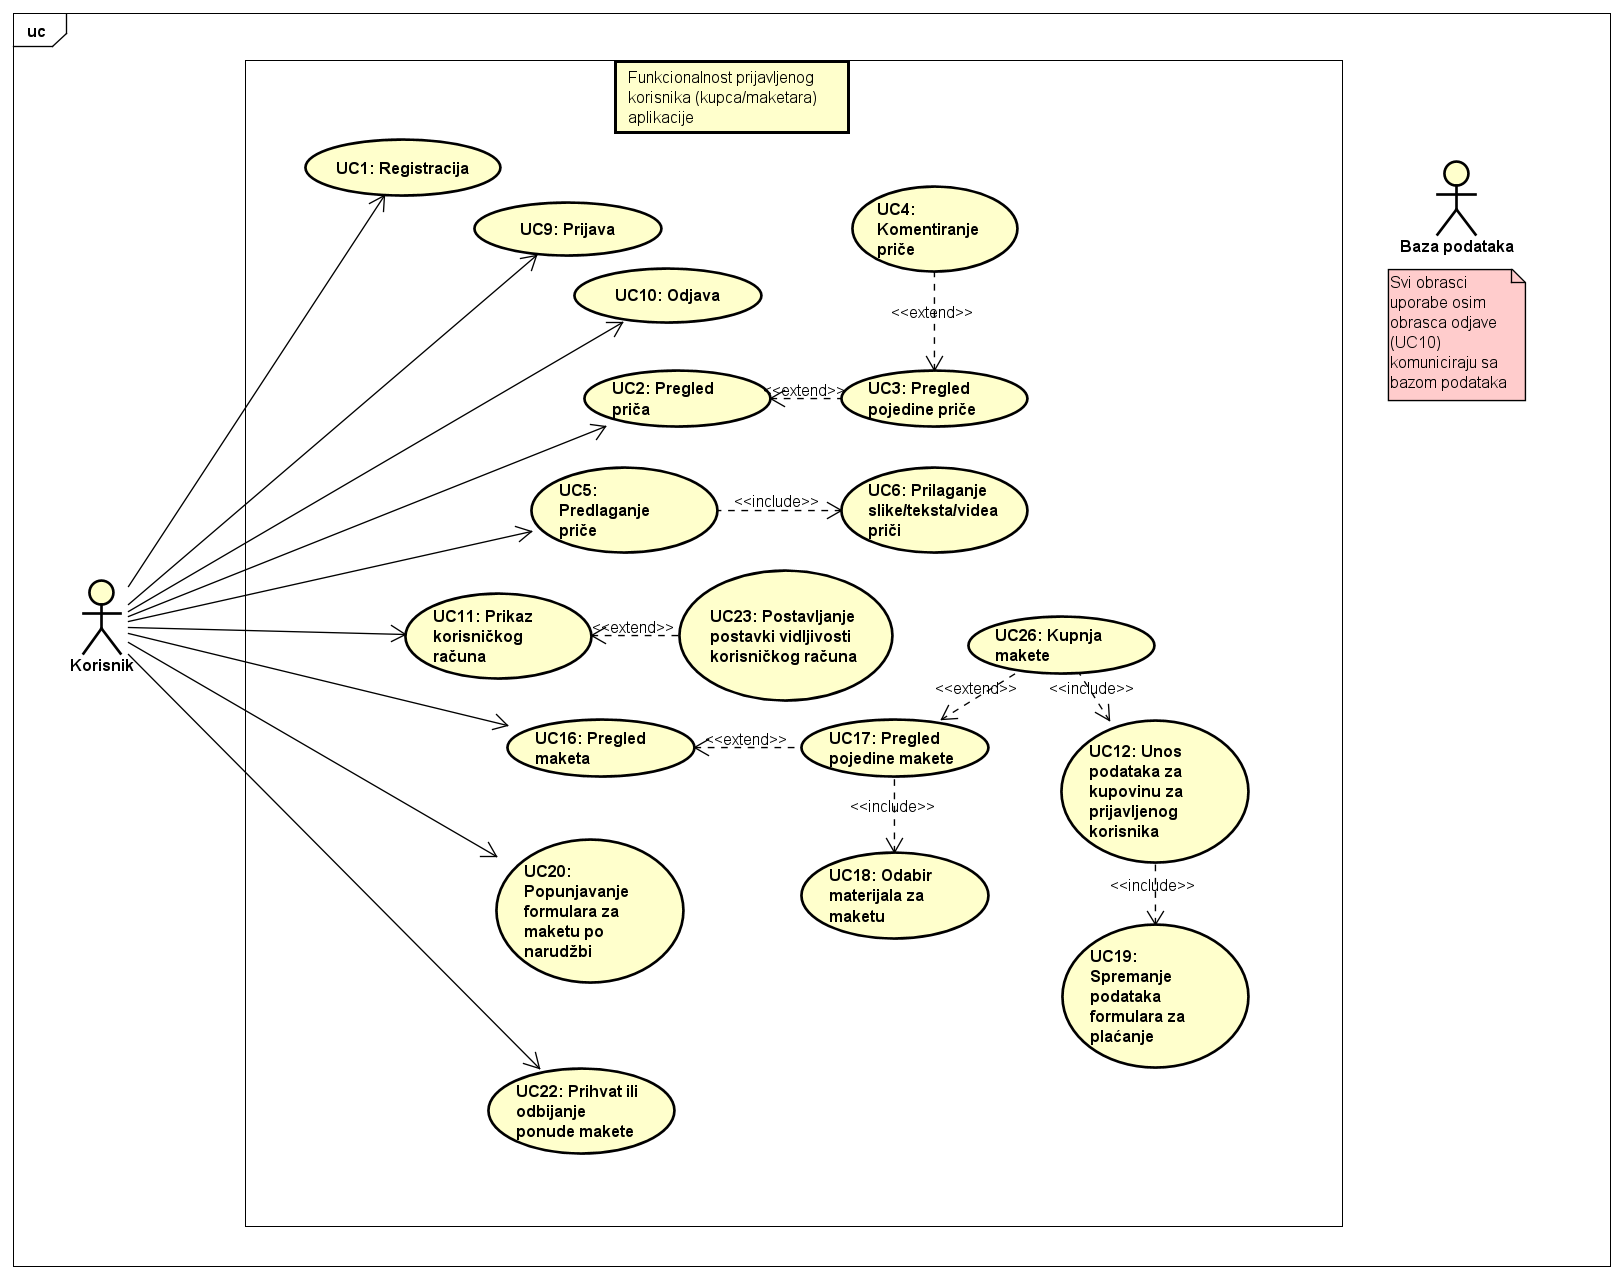
\includegraphics[width=.9\linewidth]{slike/Funkcionalnost_prijavljenog_korisnika.PNG} %veličina u odnosu na širinu linije
						\caption{Dijagram obrasca uporabe, funkcionalnost prijavljenog korisnika}
						\label{fig:obrupo1} %label mora biti drugaciji za svaku sliku
					\end{figure}
				\eject		
				
			\subsection{Sekvencijski dijagrami}
				
				\textbf{\textit{dio 1. revizije}}\\
				
				\textit{Nacrtati sekvencijske dijagrame koji modeliraju najvažnije dijelove sustava (max. 4 dijagrama). Ukoliko postoji nedoumica oko odabira, razjasniti s asistentom. Uz svaki dijagram napisati detaljni opis dijagrama.}
				\eject
	
		\section{Ostali zahtjevi}
		
			\textbf{\textit{dio 1. revizije}}\\
		 
			 \textit{Nefunkcionalni zahtjevi i zahtjevi domene primjene dopunjuju funkcionalne zahtjeve. Oni opisuju \textbf{kako se sustav treba ponašati} i koja \textbf{ograničenja} treba poštivati (performanse, korisničko iskustvo, pouzdanost, standardi kvalitete, sigurnost...). Primjeri takvih zahtjeva u Vašem projektu mogu biti: podržani jezici korisničkog sučelja, vrijeme odziva, najveći mogući podržani broj korisnika, podržane web/mobilne platforme, razina zaštite (protokoli komunikacije, kriptiranje...)... Svaki takav zahtjev potrebno je navesti u jednoj ili dvije rečenice.}
			 
			 
			 
	
	\chapter{Arhitektura i dizajn sustava}
		
		\textbf{\textit{dio 1. revizije}}\\

		\textit{ Potrebno je opisati stil arhitekture te identificirati: podsustave, preslikavanje na radnu platformu, spremišta podataka, mrežne protokole, globalni upravljački tok i sklopovsko-programske zahtjeve. Po točkama razraditi i popratiti odgovarajućim skicama:}
	\begin{itemize}
		\item 	\textit{izbor arhitekture temeljem principa oblikovanja pokazanih na predavanjima (objasniti zašto ste baš odabrali takvu arhitekturu)}
		\item 	\textit{organizaciju sustava s najviše razine apstrakcije (npr. klijent-poslužitelj, baza podataka, datotečni sustav, grafičko sučelje)}
		\item 	\textit{organizaciju aplikacije (npr. slojevi frontend i backend, MVC arhitektura) }		
	\end{itemize}

	
		

		

				
		\section{Baza podataka}
			
			\textbf{\textit{dio 1. revizije}}\\
			
		\textit{Potrebno je opisati koju vrstu i implementaciju baze podataka ste odabrali, glavne komponente od kojih se sastoji i slično.}
		
			\subsection{Opis tablica}
			

				\textit{Svaku tablicu je potrebno opisati po zadanom predlošku. Lijevo se nalazi točno ime varijable u bazi podataka, u sredini se nalazi tip podataka, a desno se nalazi opis varijable. Svjetlozelenom bojom označite primarni ključ. Svjetlo plavom označite strani ključ}
				
				\begin{longtabu} to \textwidth {|X[6, l]|X[6, l]|X[20, l]|}
					
					\hline \multicolumn{3}{|c|}{\textbf{korisnik - ime tablice}}	 \\[3pt] \hline
					\endfirsthead
					
					\hline \multicolumn{3}{|c|}{\textbf{korisnik - ime tablice}}	 \\[3pt] \hline
					\endhead
					
					\hline 
					\endlastfoot
					
					\cellcolor{LightGreen}IDKorisnik & INT	&  	Lorem ipsum dolor sit amet, consectetur adipiscing elit, sed do eiusmod tempor incididunt ut labore et dolore magna aliqua. Ut enim ad minim veniam 	\\ \hline
					korisnickoIme	& VARCHAR &   	\\ \hline 
					email & VARCHAR &   \\ \hline 
					ime & VARCHAR	&  		\\ \hline 
					\cellcolor{LightBlue} primjer	& VARCHAR &   	\\ \hline 
					
					
				\end{longtabu}
			
			
			\subsection{Dijagram baze podataka}
				\textit{ U ovom potpoglavlju potrebno je umetnuti dijagram baze podataka. Primarni i strani ključevi moraju biti označeni, a tablice povezane. Bazu podataka je potrebno normalizirati. Podsjetite se kolegija "Baze podataka".}
			
			\eject
			
			
		\section{Dijagram razreda}
		
			\begin{figure}[H]
						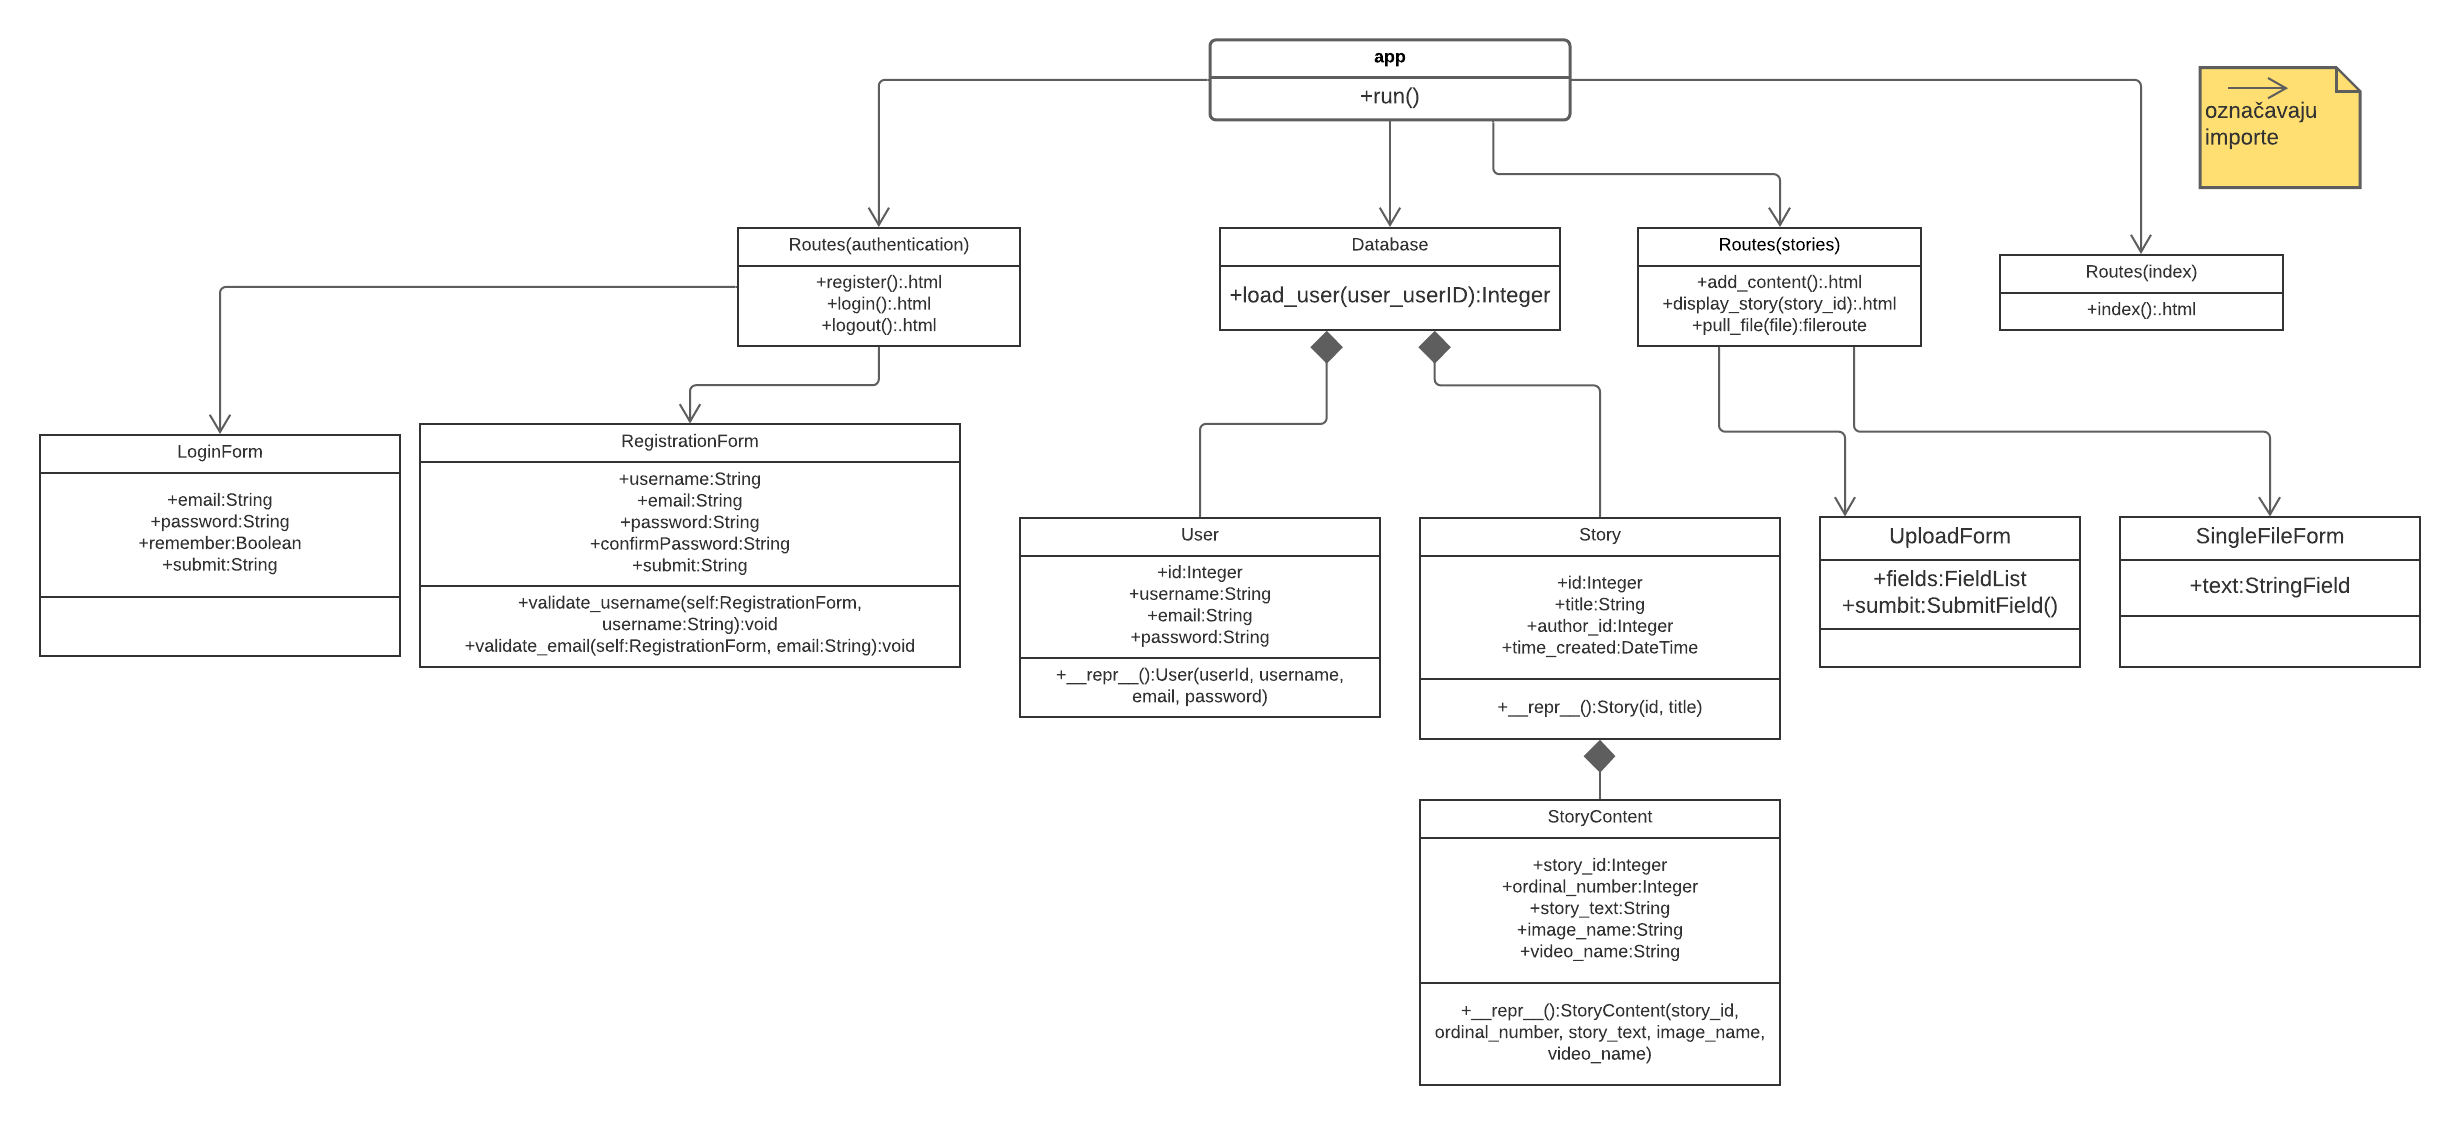
\includegraphics[width=.9\linewidth]{dijagrami/UML_class.PNG} %veličina u odnosu na širinu linije
						\caption{Dijagram razreda generičke funkcionalnosti}
						\label{fig:diraz1} %label mora biti drugaciji za svaku sliku
					\end{figure}
		
		\section{Dijagram stanja}
			
			
			\textbf{\textit{dio 2. revizije}}\\
			
			\textit{Potrebno je priložiti dijagram stanja i opisati ga. Dovoljan je jedan dijagram stanja koji prikazuje \textbf{značajan dio funkcionalnosti} sustava. Na primjer, stanja korisničkog sučelja i tijek korištenja neke ključne funkcionalnosti jesu značajan dio sustava, a registracija i prijava nisu. }
			
			
			\eject 
		
		\section{Dijagram aktivnosti}
			
			\textbf{\textit{dio 2. revizije}}\\
			
			 \textit{Potrebno je priložiti dijagram aktivnosti s pripadajućim opisom. Dijagram aktivnosti treba prikazivati značajan dio sustava.}
			
			\eject
		\section{Dijagram komponenti}
		
			\textbf{\textit{dio 2. revizije}}\\
		
			 \textit{Potrebno je priložiti dijagram komponenti s pripadajućim opisom. Dijagram komponenti treba prikazivati strukturu cijele aplikacije.}
	\chapter{Implementacija i korisničko sučelje}
		
		
		\section{Korištene tehnologije i alati}
		
			\textbf{\textit{dio 2. revizije}}
			
			 \textit{Detaljno navesti sve tehnologije i alate koji su primijenjeni pri izradi dokumentacije i aplikacije. Ukratko ih opisati, te navesti njihovo značenje i mjesto primjene. Za svaki navedeni alat i tehnologiju je potrebno \textbf{navesti internet poveznicu} gdje se mogu preuzeti ili više saznati o njima}.
			
			
			\eject 
		
	
		\section{Ispitivanje programskog rješenja}
			
			\textbf{\textit{dio 2. revizije}}\\
			
			 \textit{U ovom poglavlju je potrebno opisati provedbu ispitivanja implementiranih funkcionalnosti na razini komponenti i na razini cijelog sustava s prikazom odabranih ispitnih slučajeva. Studenti trebaju ispitati temeljnu funkcionalnost i rubne uvjete.}
	
			
			\subsection{Ispitivanje komponenti}
			\textit{Potrebno je provesti ispitivanje jedinica (engl. unit testing) nad razredima koji implementiraju temeljne funkcionalnosti. Razraditi \textbf{minimalno 6 ispitnih slučajeva} u kojima će se ispitati redovni slučajevi, rubni uvjeti te izazivanje pogreške (engl. exception throwing). Poželjno je stvoriti i ispitni slučaj koji koristi funkcionalnosti koje nisu implementirane. Potrebno je priložiti izvorni kôd svih ispitnih slučajeva te prikaz rezultata izvođenja ispita u razvojnom okruženju (prolaz/pad ispita). }
			
			
			
			\subsection{Ispitivanje sustava}
			
			 \textit{Potrebno je provesti i opisati ispitivanje sustava koristeći radni okvir Selenium\footnote{\url{https://www.seleniumhq.org/}}. Razraditi \textbf{minimalno 4 ispitna slučaja} u kojima će se ispitati redovni slučajevi, rubni uvjeti te poziv funkcionalnosti koja nije implementirana/izaziva pogrešku kako bi se vidjelo na koji način sustav reagira kada nešto nije u potpunosti ostvareno. Ispitni slučaj se treba sastojati od ulaza (npr. korisničko ime i lozinka), očekivanog izlaza ili rezultata, koraka ispitivanja i dobivenog izlaza ili rezultata.\\ }
			 
			 \textit{Izradu ispitnih slučajeva pomoću radnog okvira Selenium moguće je provesti pomoću jednog od sljedeća dva alata:}
			 \begin{itemize}
			 	\item \textit{dodatak za preglednik \textbf{Selenium IDE} - snimanje korisnikovih akcija radi automatskog ponavljanja ispita	}
			 	\item \textit{\textbf{Selenium WebDriver} - podrška za pisanje ispita u jezicima Java, C\#, PHP koristeći posebno programsko sučelje.}
			 \end{itemize}
		 	\textit{Detalji o korištenju alata Selenium bit će prikazani na posebnom predavanju tijekom semestra.}
			
			\eject 
		
		
		\section{Dijagram razmještaja}
			
			 Dijagram razmještaja je strukturni statički UML dijagram koji opisuje topologiju sustava i usredotočen je na odnos sklopovskih i programskih dijelova. Postoji više vrsta dijagrama razmještaja, a ovdje se koristi specifikacijski dijagram razmještaja kako bi se prije navedeni odnos prikazao. Za ostvarenje ove aplikacije se koristi arhitektura "klijent - poslužitelj", a komunikacija se odvija protokolom HTTP. Na klijentskoj strani se nalazi web preglednik pomoću kojeg korisnik pristupa poslužitelju, odnosno šalje HTTP zahtjeve i prima HTTP odgovore. Poslužiteljska strana je nešto složenija te se ona sastoji od web poslužitelja na koji pristižu HTTP zahtjevi i poslužitelja baze podataka kojem web poslužitelj pristupa i iz kojeg uzima, uređuje ili sprema podatke.
			 
			 \begin{figure}[H]
			 	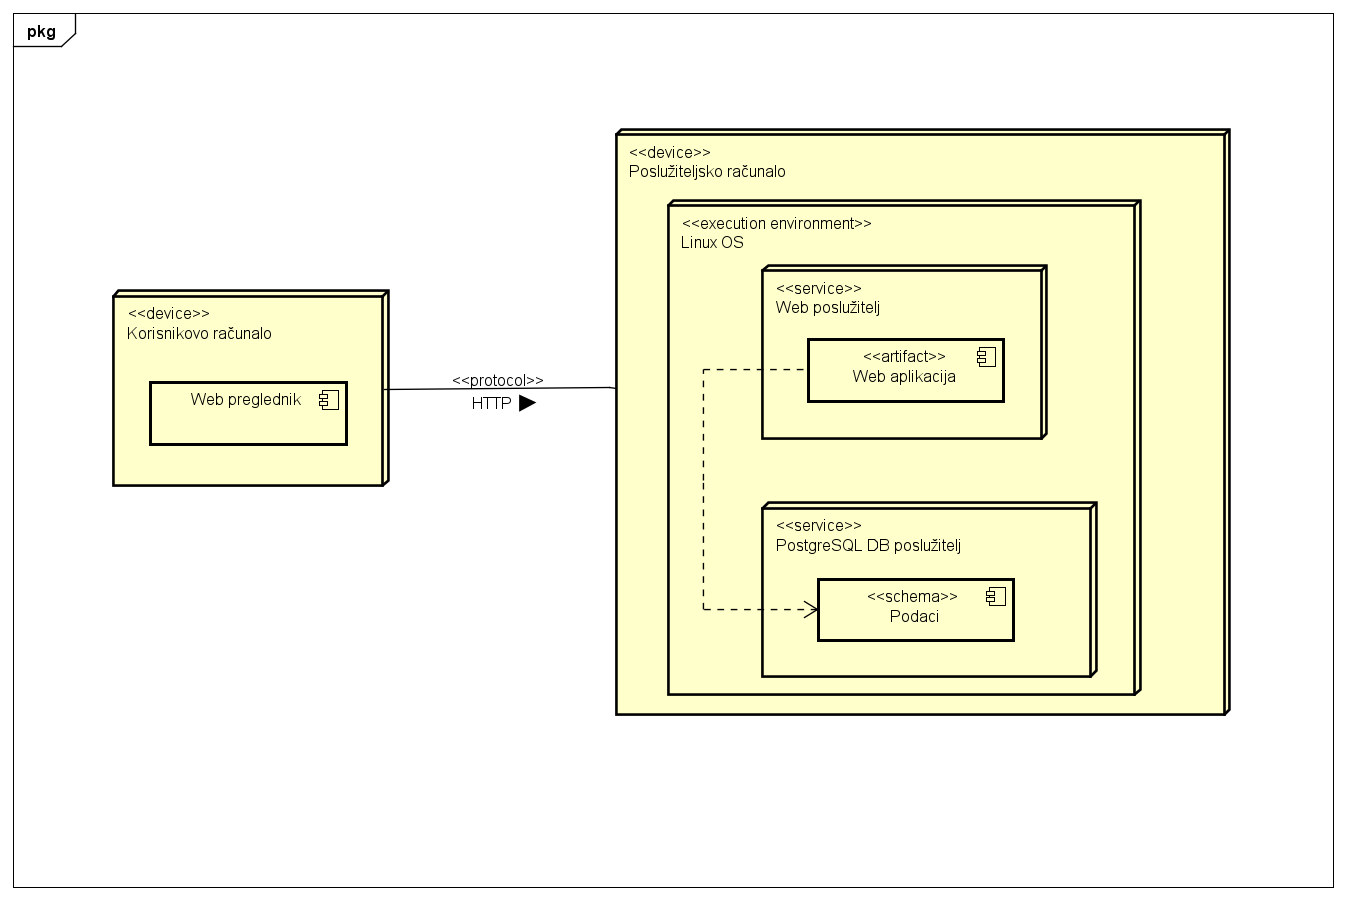
\includegraphics[width=1\linewidth]{slike/Dijagram_razmjestaja.PNG} %veličina u odnosu na širinu linije
			 	\caption{Dijagram razmještaja}
			 	\label{fig:dijraz} %label mora biti drugaciji za svaku sliku
			 \end{figure}
			
			\eject 
		
		\section{Upute za puštanje u pogon}
		
			\textbf{\textit{dio 2. revizije}}\\
		
			 \textit{U ovom poglavlju potrebno je dati upute za puštanje u pogon (engl. deployment) ostvarene aplikacije. Na primjer, za web aplikacije, opisati postupak kojim se od izvornog kôda dolazi do potpuno postavljene baze podataka i poslužitelja koji odgovara na upite korisnika. Za mobilnu aplikaciju, postupak kojim se aplikacija izgradi, te postavi na neku od trgovina. Za stolnu (engl. desktop) aplikaciju, postupak kojim se aplikacija instalira na računalo. Ukoliko mobilne i stolne aplikacije komuniciraju s poslužiteljem i/ili bazom podataka, opisati i postupak njihovog postavljanja. Pri izradi uputa preporučuje se \textbf{naglasiti korake instalacije uporabom natuknica} te koristiti što je više moguće \textbf{slike ekrana} (engl. screenshots) kako bi upute bile jasne i jednostavne za slijediti.}
			
			
			 \textit{Dovršenu aplikaciju potrebno je pokrenuti na javno dostupnom poslužitelju. Studentima se preporuča korištenje neke od sljedećih besplatnih usluga: \href{https://aws.amazon.com/}{Amazon AWS}, \href{https://azure.microsoft.com/en-us/}{Microsoft Azure} ili \href{https://www.heroku.com/}{Heroku}. Mobilne aplikacije trebaju biti objavljene na F-Droid, Google Play ili Amazon App trgovini.}
			
			
			\eject 
	\chapter{Zaključak i budući rad}		
		 \noindent Projektni zadatak naše grupe sastojao se od izrade web aplikacije za omogučavanje prodaje maketa, koja je trebala omogučiti stvaranje profila te zatraživanje izrade prilagođenih maketa uz posebne cijene.Prvi dio izrade projekta sastojao se od formiranja grupe, dobivanja zadatka,dokumentacije i implementacije generičkih funkcionalnosti. U prvom dijelu, bilo je važno izraditi specifikacije zadatka pomoću obrazaca i dijagrama, što je dalo okvir za daljnji razvoj projekta. Takoder, trebali smo odrediti koje će se tehnologije koristiti i upoznati se s njima. Osnovna podjela posla bila je u podtimovima za backend i frontend, te raspodijeliti dijelove dokumentacije za svakog člana.

		\noindent U drugom dijelu, kroz drugi ciklus semestra, fokus je bio na implementacji ostalih funkcionalnosti aplikacije, što smo radili samostalno ili u podtimovima, uz pisanje ostatka dokumentacije i testiranje projekta. Za rad na projektu posebno važna je bila organizacija i komunikacija u timu,te podjela posla i upravljanje vremenom. Komunikacija je ostvarena putem Whatsappa, gdje smo se međusobno obaviještavali o napretku i problemima sa zadatcima koje treba obaviti.Sudjelovanje na ovom projektu bilo je vrijedno iskustvo, korisno za razvoj vještina rada u timu, vremenske organiziranosti i koordinacije zadataka, kao i usvajanje novih tehnologija potrebnih za izradu aplikacije. Stečene vještine bit će veoma korisne na ostatku studija i u budućem radu.

		
		 \textit{Potrebno je točno popisati funkcionalnosti koje nisu implementirane u ostvarenoj aplikaciji.}
		
		\eject 
	\chapter*{Popis literature}
		\addcontentsline{toc}{chapter}{Popis literature}
		\begin{enumerate}
			
			
			\item  Programsko inženjerstvo, FER ZEMRIS, \url{http://www.fer.hr/predmet/proinz}
			
			\item  I. Sommerville, "Software engineering", 8th ed, Addison Wesley, 2007.
			
			\item  T.C.Lethbridge, R.Langaniere, "Object-Oriented Software Engineering", 2nd ed. McGraw-Hill, 2005.
			
			\item  I. Marsic, Software engineering book``, Department of Electrical and Computer Engineering, Rutgers University, \url{http://www.ece.rutgers.edu/~marsic/books/SE}
			
			\item  The Unified Modeling Language, \url{https://www.uml-diagrams.org/}
			
			\item  Astah Community, \url{http://astah.net/editions/uml-new}
		\end{enumerate}
		
		 
	
	
	\begingroup
	\renewcommand*\listfigurename{Indeks slika i dijagrama}
	%\renewcommand*\listtablename{Indeks tablica}
	%\let\clearpage\relax
	\listoffigures
	%\vspace{10mm}
	%\listoftables
	\endgroup
	\addcontentsline{toc}{chapter}{Indeks slika i dijagrama}


	
	\eject 
		
	\chapter*{Dodatak: Prikaz aktivnosti grupe}
		\addcontentsline{toc}{chapter}{Dodatak: Prikaz aktivnosti grupe}
		
		\section*{Dnevnik sastajanja}
		
		\textbf{\textit{Kontinuirano osvježavanje}}\\
		
		 \textit{U ovom dijelu potrebno je redovito osvježavati dnevnik sastajanja prema predlošku.}
		
		\begin{packed_enum}
			\item  sastanak
			
			\item[] \begin{packed_item}
				\item Datum: 14. listopada 2020.
				\item Prisustvovali: B.Antunović, T.Brstilo, L.Cigula,V.Jukanović, M.Marošević, M.Piskur, T.Rončević
				\item Teme sastanka:
				\begin{packed_item}
					\item  odabir objektno orijentiranog programskog jezika (Python 3)
					\item  odabir web frameworka (Flask)
					\item  rasprava vezana uz opće probleme izvođenja zadatka
					\item  postavljanje GitLab repozitorija
					\item  dogovor o strukturiranju repozitorija te interna pravila vezana uz commit
				\end{packed_item}
			\end{packed_item}
			
			\item  sastanak
			\item[] \begin{packed_item}
				\item Datum: 21. listopada 2020.
				\item Prisustvovali: B.Antunović, T.Brstilo, L.Cigula,V.Jukanović, M.Marošević, M.Piskur, T.Rončević
				\item Teme sastanka:
				\begin{packed_item}
					\item  odabir platforme za praćenje projekta i kooperaciju (Miro)
					\item  diskusija vezana uz interna pravila te način praćenja unutar alata
					\item  gruba podjela poslova na back-end i front-end
					\item  odabir template engine-a u okviru Flaska (Jinja2)
					\item  odabir DB toolkita u okviru Pythona (SQLAlchemy)
					\item  odabir register/login funkcionalnosti kao generičke funkcionalnosti koja će biti prezentirana nastavniku
				\end{packed_item}
			\end{packed_item}
			
			\item  sastanak
			\item[] \begin{packed_item}
				\item Datum: 28. listopada 2020.
				\item Prisustvovali: B.Antunović, T.Brstilo, L.Cigula,V.Jukanović, M.Marošević, M.Piskur, T.Rončević
				\item Teme sastanka:
				\begin{packed_item}
					\item  konkretna podjela poslova u okviru grube front-end, back-end podjele na 2. sastanku
					\item  podjela izrade dokumentacije među članovima tima
					\item  opća rasprava vezana uz opseg te zahtjevnost pojedinih poslova
					\item  postavljanje internih rokova u svrhu pravovremenog rješavanja kontinuiranih problema
					\item  diskusija vezana uz poteškoće povezivanja .html stranica i aplikacije
				\end{packed_item}
			\end{packed_item}			
			
			\item  sastanak
			\item[] \begin{packed_item}
				\item Datum: 4. studenoga 2020.
				\item Prisustvovali: B.Antunović, T.Brstilo, L.Cigula,V.Jukanović, M.Marošević, M.Piskur, T.Rončević
				\item Teme sastanka:
				\begin{packed_item}
					\item  rasprava vezana uz dijagrame razreda u Flasku
					\item  opća rasprava o pojedinim segmentima dokumentacije
					\item  dogovor vezan uz back-end implementaciju
					\item  opća rasprava o index stranici te već implementiranim rješenjima
				\end{packed_item}
			\end{packed_item}	
			
			%
			
		\end{packed_enum}
		
		\eject
		\section*{Tablica aktivnosti}
		
			\textbf{\textit{Kontinuirano osvježavanje}}\\
			
			 \textit{Napomena: Doprinose u aktivnostima treba navesti u satima po članovima grupe po aktivnosti.}
					
						
			
			\begin{longtabu} to \textwidth {|X[7, l]|X[1, c]|X[1, c]|X[1, c]|X[1, c]|X[1, c]|X[1, c]|X[1, c]|}
								
				\cline{2-8} \multicolumn{1}{c|}{\textbf{}} &     \multicolumn{1}{c|}{\rotatebox{90}{\textbf{Ime Prezime voditelja }}} & \multicolumn{1}{c|}{\rotatebox{90}{\textbf{Ime Prezime }}} &	\multicolumn{1}{c|}{\rotatebox{90}{\textbf{Ime Prezime }}} &	\multicolumn{1}{c|}{\rotatebox{90}{\textbf{Ime Prezime }}} &
				\multicolumn{1}{c|}{\rotatebox{90}{\textbf{Ime Prezime }}} &
				\multicolumn{1}{c|}{\rotatebox{90}{\textbf{Ime Prezime }}} &	\multicolumn{1}{c|}{\rotatebox{90}{\textbf{Ime Prezime }}} \\ \hline 
				\endfirsthead
				
			
				\cline{2-8} \multicolumn{1}{c|}{\textbf{}} &     \multicolumn{1}{c|}{\rotatebox{90}{\textbf{Ime Prezime voditelja}}} & \multicolumn{1}{c|}{\rotatebox{90}{\textbf{Ime Prezime }}} &	\multicolumn{1}{c|}{\rotatebox{90}{\textbf{Ime Prezime }}} &
				\multicolumn{1}{c|}{\rotatebox{90}{\textbf{Ime Prezime }}} &	\multicolumn{1}{c|}{\rotatebox{90}{\textbf{Ime Prezime }}} &
				\multicolumn{1}{c|}{\rotatebox{90}{\textbf{Ime Prezime }}} &	\multicolumn{1}{c|}{\rotatebox{90}{\textbf{Ime Prezime }}} \\ \hline 
				\endhead
				
				
				\endfoot
							
				 
				\endlastfoot
				
				Upravljanje projektom 		&  &  &  &  &  &  & \\ \hline
				Opis projektnog zadatka 	&  &  &  &  &  &  & \\ \hline
				
				Funkcionalni zahtjevi       &  &  &  &  &  &  &  \\ \hline
				Opis pojedinih obrazaca 	&  &  &  &  &  &  &  \\ \hline
				Dijagram obrazaca 			&  &  &  &  &  &  &  \\ \hline
				Sekvencijski dijagrami 		&  &  &  &  &  &  &  \\ \hline
				Opis ostalih zahtjeva 		&  &  &  &  &  &  &  \\ \hline

				Arhitektura i dizajn sustava	 &  &  &  &  &  &  &  \\ \hline
				Baza podataka				&  &  &  &  &  &  &   \\ \hline
				Dijagram razreda 			&  &  &  &  &  &  &   \\ \hline
				Dijagram stanja				&  &  &  &  &  &  &  \\ \hline
				Dijagram aktivnosti 		&  &  &  &  &  &  &  \\ \hline
				Dijagram komponenti			&  &  &  &  &  &  &  \\ \hline
				Korištene tehnologije i alati 		&  &  &  &  &  &  &  \\ \hline
				Ispitivanje programskog rješenja 	&  &  &  &  &  &  &  \\ \hline
				Dijagram razmještaja			&  &  &  &  &  &  &  \\ \hline
				Upute za puštanje u pogon 		&  &  &  &  &  &  &  \\ \hline 
				Dnevnik sastajanja 			&  &  &  &  &  &  &  \\ \hline
				Zaključak i budući rad 		&  &  &  &  &  &  &  \\  \hline
				Popis literature 			&  &  &  &  &  &  &  \\  \hline
				&  &  &  &  &  &  &  \\ \hline \hline
				\textit{Dodatne stavke kako ste podijelili izradu aplikacije} 			&  &  &  &  &  &  &  \\ \hline
				\textit{npr. izrada početne stranice} 				&  &  &  &  &  &  &  \\ \hline 
				\textit{izrada baze podataka} 		 			&  &  &  &  &  &  & \\ \hline 
				\textit{spajanje s bazom podataka} 							&  &  &  &  &  &  &  \\ \hline
				\textit{back end} 							&  &  &  &  &  &  &  \\  \hline
				 							&  &  &  &  &  &  &\\  \hline
				
				
			\end{longtabu}
					
					
		\eject
		
		
		\textbf{\textit{dio 2. revizije}}\\
		
		\textit{Prenijeti dijagram pregleda promjena nad datotekama projekta. Potrebno je na kraju projekta generirane grafove s gitlaba prenijeti u ovo poglavlje dokumentacije. Dijagrami za vlastiti projekt se mogu preuzeti s gitlab.com stranice, u izborniku Repository, pritiskom na stavku Contributors.}
		
	


\end{document} %naredbe i tekst nakon ove naredbe ne ulaze u izgrađen dokument 


